\documentclass[11pt]{article}

\usepackage[preprint]{acl}

\usepackage{times}
\usepackage{latexsym}

\usepackage[T1]{fontenc}
\usepackage[utf8]{inputenc}

\usepackage{microtype}
\usepackage{inconsolata}
\usepackage{graphicx}
\usepackage{amsmath}
\usepackage{amssymb}
\usepackage{booktabs}
\usepackage{array}
\usepackage{enumitem}
\usepackage{tikz}
\usepackage{multirow}
\usepackage{float}
\usetikzlibrary{positioning,arrows.meta}
\definecolor{pastelblue}{HTML}{8FB8E8}
\definecolor{pastelorange}{HTML}{F4A582}
\definecolor{pastelgreen}{HTML}{A8DCB4}
\definecolor{pastelgray}{HTML}{CFD4D9}

\newcommand{\mask}{\ensuremath{\mathrm{m}}}
\newcommand{\keep}{\textsc{keep}}
\newcommand{\edit}{\textsc{edit}}
\newcommand{\drop}{\textsc{drop}}
\newcommand{\maskdisc}{\textsc{[mask]-disc}}
\newcommand{\Tau}{\mathrm{T}}

\title{DiffusEdit: Final Submission \\ Team Wordsmiths}

\author{
  \textbf{Tatva Agarwal\textsuperscript{*}} \\ 2024117005 \And
  \textbf{Vedant Kulkarni\textsuperscript{*\dag}} \\ 2024101140 \And
  \textbf{Bysani Vedavyas\textsuperscript{*}} \\ 2024101025 \And
  \textbf{Venya Velmurugan\textsuperscript{*}} \\ 2024114002
}

\begin{document}

\maketitle

\renewcommand{\thefootnote}{\fnsymbol{footnote}}
\footnotetext[1]{Equal contribution; authors listed alphabetically.}
\footnotetext[2]{Correspondence to \texttt{\scriptsize vedant.kulkarni@students.iiit.ac.in}.}
\renewcommand{\thefootnote}{\arabic{footnote}}
\setcounter{footnote}{0}

\begin{abstract}
Reference articles go out of date as events develop, and updating them by hand is slow. Regenerating the article with a fine-tuned language model automates the update, but trains every parameter of the model and leaves no record of which tokens changed. DiffusEdit instead edits the article in place. Small trained networks, called classifiers, read the hidden states of a frozen diffusion language model and decide which sentences to keep, edit or delete, and which tokens inside them are stale. The frozen model rewrites only the stale positions, and the system repeats the process on sentences that the rewrites themselves made wrong. Training labels come from Wiki Wrong, a synthetic benchmark of Wikipedia leads with known edits that we introduce, and evaluation measures update quality, minimality, and coverage of the cascading edits.\footnote{\scriptsize\url{https://github.com/gamemaker1/diffusedit}}\footnote{\scriptsize\url{https://huggingface.co/datasets/gamemaker1/wiki-wrong}}\footnote{\scriptsize\url{https://huggingface.co/gamemaker1/diffusedit}}\footnote{\scriptsize\url{https://huggingface.co/gamemaker1/t5edit}}
\end{abstract}

\section{Introduction}
Reference text goes out of date. A Wikipedia article about a factory fire may say that three people died and that the small death toll limited the political fallout. A week later, news reports revise the toll to forty-two. The first sentence is contradicted directly, but the second is wrong because the fact it follows from no longer holds. We call the second kind of required change a \emph{cascading edit}, a sentence that must change only because another sentence changed.

DiffusEdit updates the article in place. It is built on a frozen diffusion language model that is trained to predict masked tokens from the unmasked tokens on both sides of a token and that generates text by filling masks over several steps, so it can rewrite a span in the middle of a sentence while the rest stays fixed. The model is never trained here. Instead, small trained networks, called \emph{classifiers}, read the vectors that the frozen model computes for each token, its hidden states, and choose the stale sentences and tokens. The model infills only those positions, and the loop repeats on sentences the repairs themselves broke. In the fire example, round one masks \emph{three} and infills \emph{forty-two}, and round two rewrites the fallout sentence the first repair left unsupported.
    
\section{Task Definition}
\label{sec:problem}

An article is a sequence of sentences $A = (s_1, \dots, s_n)$, new evidence arrives as a set of text snippets $E = (e_1, \dots, e_m)$, and the system must produce an updated article $\hat{A}$ from the two alone. Faithfulness requires every claim in $\hat{A}$ to agree with the evidence and the untouched parts of the article, coverage requires every evidence fact that bears on the article to appear in $\hat{A}$, and minimality requires $\hat{A}$ to stay close to $A$.

\section{Related Work}
\label{sec:related}

Early evidence-driven correction handles one sentence or claim at a time, masks the tokens that a new fact contradicts and refills them \citep{shah-etal-2020-automatic, thorne-vlachos-2021-evidence}. Closest to us, FRUIT \citep{iv-etal-2022-fruit} defines the task this project works on, and its EDIT5 model writes the updated article left to right while copying unchanged sentences through special tokens.

EditPropBench \citep{kruthof-2026-editpropbench} measures how many required downstream changes a model finds after a planted edit, and the strongest prompted model tested misses about 30\% of them.

\citet{malmi-etal-2019-encode} edit text by tagging each token to keep it, delete it or add a phrase before it. \citet{iso-etal-2020-fact} revise a document to match facts given as triples. \citet{spangher-etal-2022-newsedits} release a corpus of news article revisions, from which \citet{panthaplackel-etal-2022-updated} update the title of a news article when the article changes. RARR \citep{gao-etal-2023-rarr} finds evidence for a model's output and revises its unsupported claims, GenAudit \citep{krishna-etal-2024-genaudit} revises or removes the claims of a response that a reference document does not support, and PEER \citep{schick-etal-2022-peer} is trained to draft, edit and explain its edits.

In diffusion language models such as LLaDA \citep{nie-etal-2025-llada} and Dream \citep{ye-etal-2025-dream}, several works reconsider tokens the sampler already committed \citep{wang-etal-2025-remasking, bie-etal-2026-llada21}. Detect, Remask, Repair \citep[DRR;][]{zou-etal-2026-detect} is a prior system that applies a diffusion model to existing text and external evidence. It scores each token of a stale summary with \maskdisc{}, a linear classification layer over the diffusion model's hidden states, then masks and infills the highest-scoring tokens, re-scoring the summary over several rounds. Our work extends this system.

\section{Contributions}
\label{sec:contributions}

DRR detects tokens that clash with the evidence on summaries of at most about ninety tokens, trains its detector on synthetic corruptions of such summaries, and fills every masked position with one token, so an edit keeps the length of its mask. DiffusEdit extends it to whole articles with the following contributions.
\begin{enumerate}[leftmargin=*,itemsep=1pt]
    \item We introduce and release Wiki Wrong, a synthetic benchmark of 15,346 Wikipedia leads with sentence labels, stale token spans, gold rewrites and cascade links, in which every edit is reversed so that a memorised fact is wrong (Section~\ref{sec:synthetic}). FRUIT-WIKI marks no stale tokens, and in a hand audit 13 of its 39 audited \edit{} labels mark sentences whose facts did not change (Section~\ref{sec:fruit}).
    \item A sentence classifier and a staleness classifier over the hidden states of a frozen diffusion model, in which the staleness classifier attends over the states of the evidence tokens (Sections~\ref{sec:method} and~\ref{sec:focus}).
    \item Infilling rules that let a frozen model shorten, lengthen or delete a span, copy a value from the evidence, and leave correct words unchanged, and a learned ranking of the candidates. Infilling alone fills every mask with one token and cannot remove a span.
    \item A loop of up to three rounds that repairs the cascade sentences that the first repairs leave wrong, with a consequence classifier and two other cascade detectors compared on the test articles that contain a cascade. A cascade sentence clashes only with another sentence that changed, so scoring tokens against the evidence has no signal for it.
\end{enumerate}

\begin{figure*}[t]
\centering
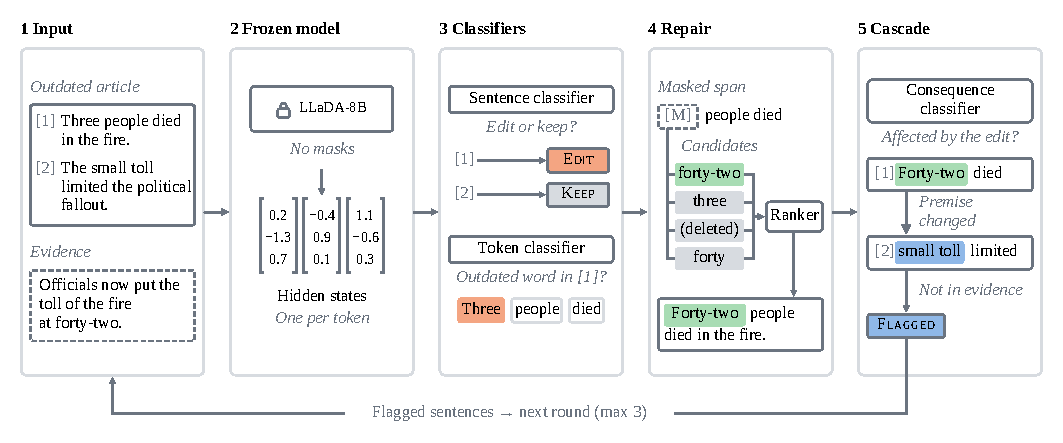
\includegraphics[width=\textwidth]{figures/system.pdf}
\caption{One round of DiffusEdit on the fire example. Orange marks the token the staleness classifier scores as stale, green the value the evidence supplies, and blue the sentence the consequence classifier flags for the next round.}
\label{fig:pipeline}
\end{figure*}

\section{Methodology}
\label{sec:method}

DiffusEdit repairs an article in rounds (Figure~\ref{fig:pipeline}). In each round the frozen model runs once over the evidence and the article, the classifiers label the sentences to change and the stale tokens in them, the model fills in only those tokens to give several candidate sentences, a ranker picks one, and a cascade detector flags the sentences that the repairs may have broken, which become the next round. Table~\ref{tab:choices} in the appendix lists the fixed values of the method and the reason for each.

\subsection{Shared Forward Pass}
The input is the evidence passages followed by the article. LLaDA-8B-Base \citep{nie-etal-2025-llada} runs once over this sequence with no mask. Because it reads in both directions, the state of every token reflects the whole sequence, evidence included. We keep the \emph{hidden state} of every token at every block, meaning the vector that the model computes for that token at that block (of length 4,096). The classifiers read the states of the article tokens, and the staleness classifier also reads the states of the evidence tokens. One pass serves all classifiers, which are trained on these states while LLaDA's weights stay fixed. For a sentence $s_j$ with token positions $I_j$, the sentence vector is the mean of its token states at block $b$:
\begin{equation}
u_j^{(b)} = \frac{1}{|I_j|}\sum_{i \in I_j} h_i^{(b)}.
\end{equation}

\subsection{Sentence Classifier}
The sentence classifier labels every article sentence \keep{}, \edit{} or \drop{}. It is a linear layer on the sentence vector at block 24 of the 32 blocks,
\begin{equation}
p_j = \mathrm{softmax}\big(W\,u_j^{(24)} + b\big),
\end{equation}
trained with cross-entropy on the train split. The label with the highest probability is taken, except that a sentence whose most probable label is \drop{} is deleted only if that probability is at least $\tau_d = 0.8$, a threshold set on validation, and is labelled \edit{} otherwise. Block 24 is used because its validation macro-F1 is 0.844, against 0.717 for block 32 (Table~\ref{tab:classifiers}). A \keep{} sentence is left alone, an \edit{} sentence goes on to token scoring, and a \drop{} sentence is deleted.

\subsection{Token Staleness Classifier}
For each token of an \edit{} sentence, the staleness classifier, which reads block 32, outputs $\pi_i \in [0,1]$, the probability that the token is stale. A token is stale when the evidence states a different value in its place, so the classifier compares the token with the evidence through attention. For an article token with state $h_i$ and evidence tokens with states $e_1, \dots, e_M$, the classifier forms a query, keys and values,
\begin{equation}
q_i = W_q h_i, \quad k_m = W_k e_m, \quad v_m = W_v e_m,
\end{equation}
with a learned \emph{null} slot $k_0, v_0$ that stands for no evidence, so that a token the evidence does not mention has somewhere to place its weight. The attention weights and the attention output are
\begin{equation}
\alpha_{im} = \operatorname*{softmax}_{m = 0, \dots, M} \frac{q_i^\top k_m}{\sqrt{r}}, \qquad o_i = \sum_{m=0}^{M} \alpha_{im} v_m ,
\end{equation}
where the vectors have width 256, split over four heads of width $r = 64$, and $o_i$ joins the outputs of the four heads. The token state is mapped to the same width by $t_i = W_t h_i$, and a small feed-forward network compares $t_i$ with $o_i$:
\begin{equation}
\pi_i = \sigma\big(\mathrm{MLP}([\,t_i;\ o_i;\ t_i \odot o_i;\ |t_i - o_i|\,])\big).
\end{equation}
Figure~\ref{fig:attention} shows the mechanism on a test sentence, and Section~\ref{sec:focus} measures where the weight falls. This extends \maskdisc{} \citep{zou-etal-2026-detect}, which scores tokens with a linear layer. The classifier is trained with binary cross-entropy on the train split. A source token is labelled stale if a word-level comparison with the gold rewrite marks it as changed.

\begin{figure}[t]
\centering
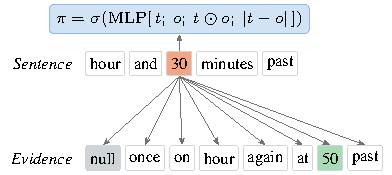
\includegraphics[width=0.92\columnwidth]{figures/attention.pdf}
\caption{The staleness classifier on the test sentence ``There are two updates an hour, at the top of the hour and 30 minutes past'', whose gold update replaces \emph{30} by \emph{50}. The query of the token \emph{30} is scored against every evidence token and the null slot. Evidence words stand in for LLaDA tokens, and some are left out. The arrows mark the comparison and are not measured weights.}
\label{fig:attention}
\end{figure}

\subsection{Masking Policy}
The masking policy turns the token scores of an \edit{} sentence into masks. Tokens with $\pi_i \ge \tau$ are masked, with $\tau = 0.85$:
\begin{equation}
M = \{\, i : \pi_i \ge \tau \,\}.
\end{equation}
If $M$ is empty, the classifier's \edit{} label is trusted and the top fifth of the sentence by score is masked. If $M$ covers more than half of the sentence, only the highest-scoring half is kept, because such a sentence is closer to a rewrite than a repair. A single unmasked token between two masked tokens is masked too, so that a fragmented score gives one region to rewrite, and each masked token is widened to its whole word.

Runs of adjacent masks form \emph{spans}. A token can be masked at most three times over all rounds, which is the re-masking cap of \citet{yao-2026-remask} and stops the loop from masking the same span forever.

\subsection{Variable-Length Infilling}
A diffusion model fills every mask with exactly one token, so a span of $n$ masks gives $n$ tokens, but a correct update can be shorter, longer or empty. Models that let the masked region grow or shrink exist \citep{wu-etal-2026-dreamon, zhang-etal-2025-ddot}, but they need the diffusion model to be trained, and ours stays frozen. We therefore fill each span at four lengths,
\begin{equation}
\Lambda(n) = \{\,0,\ \lceil n/2\rceil,\ n,\ n+2\,\},
\end{equation}
which delete, shorten, keep and lengthen it. At each length LLaDA fills the masks greedily over eight steps, with the whole evidence and article as context. Every filled sentence is a \emph{candidate}, and the candidates of one sentence form its \emph{pool}.

A greedy fill holds only the tokens that LLaDA ranks highest, so it can miss a new value that LLaDA finds unlikely in the span. Each span therefore also receives up to four \emph{evidence-copy} candidates, which put a phrase of the evidence into the span word for word. The phrases are the named entities that spaCy finds in the evidence and that the sentence does not already contain. They are limited to the entity type of the masked text, such as a date for a masked date, or to names or numbers when the masked text is not part of an entity. If more than four phrases qualify, each phrase is placed in the span as a run of masks of its token length, LLaDA predicts those masks, and the phrase is scored by the mean log-probability of its own tokens. The four phrases with the highest score become candidates.

\subsection{Infilling Rules}
The four rules below and the evidence-copy candidates together are the \emph{infilling rules}. The setting that uses them is called \emph{with infilling rules}, and the setting without them \emph{without infilling rules}.
\begin{itemize}[leftmargin=*,itemsep=1pt]
    \item \textbf{Edit penalty.} A candidate loses $0.1$ times its word edit distance from the sentence before repair, so that it is charged for every changed word \citep{chen-etal-2022-converge}.
    \item \textbf{Rejection rule.} A candidate loses $100$ if it contains an entity, meaning a capitalised word or a number, that occurs in neither the evidence nor the sentence before repair. If every candidate is rejected, the best of them still wins.
    \item \textbf{Evidence veto.} A span whose words all occur somewhere in the evidence is left as-is, because the evidence does not contradict it.
    \item \textbf{Span cap.} A sentence whose mask has more than two spans is left unrepaired, because such masks were mostly wrong.
\end{itemize}

\subsection{Ranking}
\paragraph{Heuristic ranking}
The heuristic ranking combines a fluency score and an agreement score. The pseudo-log-likelihood (PLL) measures fluency. It is the mean log-probability that LLaDA gives each token of the sentence when that token alone is masked. $\mathrm{Ent}$ measures agreement with the evidence. It is the probability that a VitaminC fact verifier \citep{schuster-etal-2021-vitaminc} gives to the best evidence passage supporting the sentence. A candidate $c$ with sentence $s_c$ scores
    \begin{equation}
    \begin{aligned}
    \mathcal{R}(c) = &\; 0.5\,\mathrm{PLL}(s_c) + 0.5\,\mathrm{Ent}(s_c) \\
                     &- 0.1\,d(s_c, s) - 100\,[\mathrm{rej}(c)]
    \end{aligned}
  	\end{equation}
where $d$ is the word edit distance to the sentence $s$ before repair, and $[\mathrm{rej}(c)]$ is $1$ if the candidate is rejected and $0$ otherwise. A deletion wins only when its score is at least $0.1$ above the best rewrite, because removing a span also removes the claim that the verifier would have checked.

\paragraph{Learned ranking}
The learned ranking replaces the heuristic score with a gradient-boosted tree classifier, as one fixed formula did not cover all cases. Every candidate is a whole sentence, so the logged pools can be ranked again without another model pass. Each candidate gets its PLL and Ent scores with their ranks in the pool, the ratio of its fill length to the span length, its word edit distance and ROUGE-L to the source, the counts of capitalised words and numbers it adds or drops, split by whether the evidence holds them, and the sampler's confidence. The unchanged source joins every pool as one more candidate, so the ranking can leave a sentence as it is. The classifier is fit to predict whether a candidate has the best ROUGE-L of its pool, and the candidate with the highest predicted probability is the output. It holds 200 trees of at most 15 leaves each and is fit on the candidate pools of 200 validation articles.

\subsection{Rounds and Cascades}
After each round a cascade detector flags \emph{cascade} sentences, the cascading edits of the introduction, outside the repaired set, and the next round repairs them. The loop runs at most three rounds, and every round starts with a fresh forward pass, because the repairs changed the text that the old states describe. A loop with no detector stops after one round.

\paragraph{Consequence classifier}
A small trained network scores whether a sentence $s_k$ must change because the repaired sentence $s_j$ did. It reads the pooled states at block 32 of $s_j$ after its repair and of $s_k$ before it, and flags the pair when the score exceeds $\tau_c = 0.35$. Block 32 is the only block tried for this classifier, and its validation AUROC there is 0.945 (Table~\ref{tab:classifiers}):
\begin{equation}
g_{jk} = \sigma\big(\mathrm{MLP}([\,u_j;\ u_k;\ u_j \odot u_k;\ |u_j - u_k|\,])\big).
\label{eq:consequence}
\end{equation}
The product and the absolute difference give the network similarity signals that it would otherwise have to learn.

\paragraph{Staleness delta}
This flags a sentence whose staleness scores rise after the round.

\paragraph{Edited as evidence}
This appends the repaired sentences to the evidence, so that the next pass covers them, and flags the sentences that the classifier then labels \edit{}.



\section{Data}
\label{sec:data}

\subsection{FRUIT}
\label{sec:fruit}
FRUIT-WIKI \citep{iv-etal-2022-fruit} pairs two snapshots of a Wikipedia article and marks every sentence that changed between them as an update. Between two snapshots, editors also reword sentences for style and move sentences out of the lead into other sections, and neither change has evidence behind it. Such a sentence carries the same \edit{} or \drop{} label as one whose fact changed. Three co-authors labelled 100 training sentences from 23 randomly drawn articles against the two snapshots, and 13 of the 39 \edit{} labels with a majority verdict marked sentences whose facts had not changed. The evidence is also often missing. In a first run on 200 held-out articles, only 57 of the 338 \edit{} sentences whose gold rewrite adds words had those words anywhere in the source article or the evidence, so most gold updates cannot be reached from the input. A classifier trained on these labels is trained to call a rewording stale, and a repair step scored on them is asked for facts it is not given. FRUIT was therefore replaced by Wiki Wrong, a synthetic benchmark in which every \edit{} changes a value, the evidence states the new value, and the stale tokens are known.

\subsection{Wiki Wrong}
\label{sec:synthetic}
We introduce Wiki Wrong, which starts from 30,000 English Wikipedia leads, one article per record. In each lead a sentence is chosen for an edit with probability 0.35 and for a deletion with probability 0.10, independently of the other sentences, so that the position of a sentence carries no information about its label. After the checks below, 29\% of the sentences are \edit{} and 7\% \drop{}, against 42\% and 12\% in the collated FRUIT training split. An edited sentence has one to three values replaced, so that a sentence can have more than one stale span: a named entity by an entity of the same type and shape drawn from other articles, so that the replacement reads as naturally as the original, and a year or an integer by a nearby one, so that the change is not visible from the magnitude alone. With probability 0.25 an edit also receives a cascade, a second sentence whose value follows from the first, such as a century from a year, an age from a birth date, a demonym from a country, or pronouns from a name.

Evidence passages are written by Claude Sonnet agents from a fixed brief, as excerpts of other documents such as news reports and reference entries, and an article is kept only if every new value of a direct edit occurs in a passage about that sentence, no passage holds an old value, every deleted sentence has a passage that retracts it, no passage copies seven consecutive words of a sentence, so that a string match between the passage and the article cannot stand in for reading the evidence, and no passage supports a cascade sentence, so that a cascade can be found only through the sentence it depends on. The sentence labels, the stale spans and the gold rewrites follow from the construction, so the label noise of FRUIT is absent.

LLaDA-8B-Base has read Wikipedia in pretraining, so a lead with a wrong value clashes with what its weights hold, and a classifier or an infilling run can find the stale text without the evidence. The direction of every edit is therefore reversed. The real Wikipedia sentence is the outdated source, the mutated sentence is the gold update, and the evidence states the mutated values. A model that reproduces a memorised fact is wrong under the reversal, and the gold update can be reached only through the evidence.


The classifiers are fit on the training split, every threshold and every design choice is set on the validation split, and the test split is scored once per configuration. The size of each split is given in Table~\ref{tab:splits}. Sentence-level results are reported on all 1,670 \edit{} sentences of the 901 test articles that have at least one supported \edit{} sentence, meaning one whose gold rewrite adds no word that is absent from both the evidence and the source sentence; 1,420 of the 1,670 are supported themselves. The repair step was run on test twice: once without the infilling rules, whose score motivated the rules, which were then designed on 200 validation articles and selected on a disjoint 200, and once with them. The rule ablations run on a seeded sample of 300 of the 901 articles, and the loop ablations on a seeded sample of 300 of the 1,602 test articles. LLaDA-8B-Base runs in bfloat16 and is never trained, and the classifiers together hold 12.9M parameters.

\subsection{Baselines and Controls}
The common baseline for this task is copying the source unchanged. The single round stops after the first round with no cascade detector, which is similar to a single-pass setting of DRR \citep{zou-etal-2026-detect}, so the difference to the full loop is the effect of the extra rounds. Every loop and article-level result uses the heuristic ranking, because the learned ranking was fit on logged pools after the loops had run. The Flan-T5 editor is \texttt{flan-t5-large}, 780M parameters, fully fine-tuned on the 12,180 training articles to write the updated article from the outdated article and the evidence in the format of EDIT5 \citep{iv-etal-2022-fruit}. It is the upper bound. It trains all of its parameters on the full training split, and its output carries no record of which tokens changed. Oracle masks give the infilling step the gold stale tokens, so the gap to the predicted masks is the cost of the staleness classifier. Gold sentence labels given to the loop bound what better labels and detection together could add.

\subsection{Metrics}
Sentence-level scores compare the output sentence with the gold rewrite by ROUGE-L F1. Exact match counts outputs equal to the gold rewrite after case and whitespace normalisation. New-value recall is the share of new values that occur in the output as whole words, and old-value kept is the share of old values that still occur, over old values absent from the gold update, so a lower value is better. Verifier support is the probability of SUPPORTS that the VitaminC verifier of the ranking step gives the output sentence against its best evidence passage, a check against the evidence rather than against the gold rewrite.

Article-level scores compare whole articles. UpdateROUGE-L \citep{iv-etal-2022-fruit} is ROUGE-L between the sentences of the output and of the gold article that differ from the source. \keep{} verbatim is the share of gold \keep{} sentences that appear unchanged in the output. Entity precision and recall compare the mentions, meaning named entities and numbers, of the output sentences that differ from the source with the mentions of the gold update's changed sentences. Unsupported is the count per article of output mentions that occur in neither the source article nor the evidence. Cascade ROUGE-L is UpdateROUGE-L restricted to the cascade sentences. Cascade recall is measured outside the loop: the direct edits of an article are repaired with their gold rewrites, and the recall is the share of cascade sentences that the detector then flags. The classifiers are scored with macro-F1, the mean over the three sentence labels of the harmonic mean of precision and recall, with the area under the precision-recall curve (PR-AUC) for the token labels, whose positive share is 11\%, and with the area under the receiver operating curve (AUROC), the probability that a cascade pair scores above a non-cascade pair, for the consequence pairs. Every interval is a 95\% bootstrap interval over articles, from at least 2,000 resamples of the articles with replacement.

\section{Results}
\label{sec:results}

\subsection{Classifiers}

\begin{figure}[t]
\centering
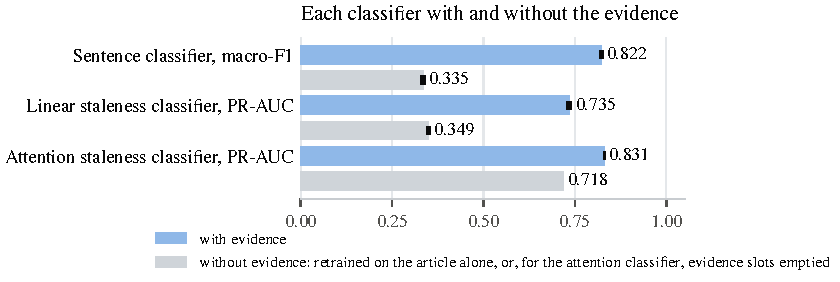
\includegraphics[width=\columnwidth]{figures/evidence.pdf}
\caption{Each classifier on the test split with its evidence and without it.}
\label{fig:evidence}
\end{figure}

Figure~\ref{fig:evidence} and Table~\ref{tab:classifiers} hold the classifier scores. The sentence classifier over LLaDA states scores above the same classifier over sentence-transformer embeddings, and the attention staleness classifier scores above the linear staleness classifier. Every classifier loses most of its score without the evidence (Figure~\ref{fig:evidence}). Over five training seeds, the standard deviation of each test score is at most 0.006 (Table~\ref{tab:classifiers}).

\subsection{Sentence Repair}

\begin{figure}[t]
\centering
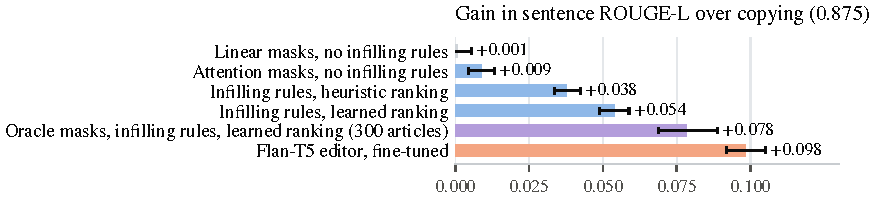
\includegraphics[width=\columnwidth]{figures/ladder.pdf}
\caption{Sentence ROUGE-L of every repair setting, from copying to the fine-tuned editor.}
\label{fig:ladder}
\end{figure}

Figure~\ref{fig:ladder} holds the gain of every repair setting over copying, Figure~\ref{fig:values} the value-level scores, and Table~\ref{tab:sentence} every sentence score. Without the infilling rules, both kinds of predicted masks stay within 0.01 of copying. The infilling rules and the learned ranking together close 55\% of the gap between copying and the Flan-T5 editor (Figure~\ref{fig:ladder}). The learned ranking keeps the old value in about half as many sentences as the heuristic ranking (Figure~\ref{fig:values}). With both systems fit on the first 500 training articles, the classifiers score 0.042 sentence ROUGE-L above the editor, with a paired 95\% interval of 0.031 to 0.053, and the editor scores as copy (Table~\ref{tab:matched}).

\subsection{Article Level}
\label{sec:article}
\begin{table*}[t]
\centering
\footnotesize
\setlength{\tabcolsep}{7pt}
\begin{tabular}{@{}llcccccc@{}}
\toprule
\textbf{Articles} & \textbf{System} & \textbf{Upd. R-L} & \textbf{Ent. P} & \textbf{Ent. R} & \keep{} \textbf{verb.} & \textbf{Unsupp.} $\downarrow$ & \textbf{Casc. R-L} \\
\midrule
\multirow{4}{*}{300 test} & Single round & 0.476 & 0.675 & 0.382 & 92.7\% & \textbf{0.19} & \\
 & Consequence loop & 0.490 & 0.665 & 0.399 & 90.7\% & 0.20 & \\
 & Flan-T5 editor & \textbf{0.911} & \textbf{0.915} & \textbf{0.885} & \textbf{97.9\%} & 0.25 & \\
 & Loop, no evidence & 0.062 & 0.116 & 0.015 & 93.7\% & 0.09 & \\
\midrule
\multirow{3}{*}{220 linked} & Single round & 0.436 & 0.866 & 0.330 & 92.9\% & \textbf{0.30} & 0.210 \\
 & Consequence loop & 0.470 & 0.847 & 0.360 & 89.8\% & 0.35 & 0.296 \\
 & Flan-T5 editor & \textbf{0.926} & \textbf{0.949} & \textbf{0.890} & \textbf{95.6\%} & 0.98 & \textbf{0.815} \\
\bottomrule
\end{tabular}
\caption{Article scores on a seeded sample of 300 test articles and on the 220 test articles with a cascade link. Ent. P and Ent. R are the precision and recall of the mentions of the changed sentences against the gold update, with precision averaged over the articles in which a system changed a sentence. Copy scores 0 UpdateROUGE-L, 100\% \keep{} verbatim and 0 unsupported mentions. Bold marks the best system in each group, leaving out the no-evidence control, which changes almost nothing.}
\label{tab:editor-article}
\end{table*}

Table~\ref{tab:editor-article} holds the article scores. On the 220 linked articles the loop adds about a third as many unsupported mentions as the editor. On the 300 test articles the two systems add a similar number, and the paired 95\% interval of that difference covers zero. The editor scores higher on UpdateROUGE-L, on entity precision and recall, and on \keep{} verbatim (Table~\ref{tab:editor-article}).

\subsection{Cascades}
\label{ssec:results_cascades}

\begin{figure*}[t]
\centering
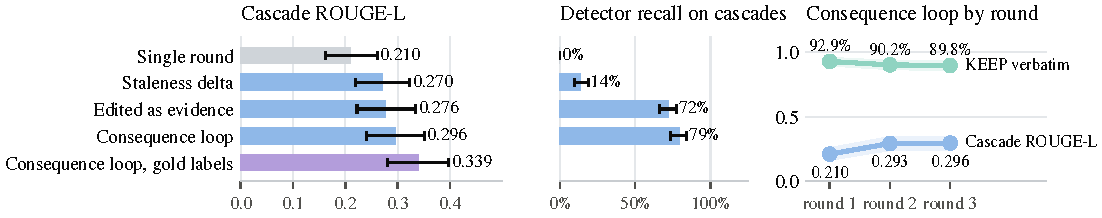
\includegraphics[width=\textwidth]{figures/cascade.pdf}
\caption{The loop on the 220 linked test articles: each detector's cascade ROUGE-L and its recall after an oracle repair, and the consequence loop after each round.}
\label{fig:cascade}
\end{figure*}

Table~\ref{tab:cascade_results} and Figure~\ref{fig:cascade} hold the loop results on the 220 linked test articles. Every detector raises cascade ROUGE-L over the single round. Among the loops with predicted labels, the consequence loop has the highest cascade ROUGE-L and detector recall, and the highest \keep{} verbatim of the three detectors (Table~\ref{tab:cascade_results}). The second round gives almost the whole cascade gain, and the third round lowers \keep{} verbatim slightly (right panel of Figure~\ref{fig:cascade}). In the logged edits of the consequence loop, 76\% of the cascade sentences enter some round and 32\% are changed in the output, against 53\% and 23\% for the single round.

\subsection{Attention over the Evidence}
\label{sec:focus}


For every token of a test \edit{} sentence whose new values occur in the evidence, 43,163 tokens in 915 articles, the attention weights of the staleness classifier were averaged over its four heads and split by whether the token is stale (Table~\ref{tab:focus}). A stale token places about seven times the uniform share of its weight on the tokens of the value that replaces it, and a token that is not stale places about three and a half times the uniform share there. The most weighted evidence token lies in the new value for 64\% of stale tokens and 23\% of other tokens, and the share is highest when the new value is a year and lowest when it is a name (Table~\ref{tab:focus}).

\section{Discussion}
\label{sec:discussion}

\paragraph{Evidence}
The measured gains depend on the evidence. Every classifier loses most of its score without the evidence (Figure~\ref{fig:evidence}), the loop without the evidence changes almost nothing (Table~\ref{tab:editor-article}), and oracle masks filled without the evidence score below copy (Table~\ref{tab:ablation-single}), because under the reversed data the memorised fact is the old value. The attention of the staleness classifier falls on the value that replaces a stale token far above the uniform share (Table~\ref{tab:focus}), so the staleness score is tied to the matching evidence tokens. The null slot receives less than 0.1\% of the weight (Table~\ref{tab:focus}), so a token that the evidence does not mention spreads its weight over the evidence instead.

\paragraph{Masks and Rules}
Without the infilling rules the repair writes the new value about as often as with them, but it reaches the gold rewrite half as often (Table~\ref{tab:sentence}), because the sampler also changes words that were correct. The infilling rules raise the score mainly by leaving those words unchanged, and the learned ranking raises it further by choosing among the same candidates, keeping the old value in about half as many sentences (Figure~\ref{fig:values}). Oracle masks close about half of the remaining gap to the editor on the 300-article sample (Figure~\ref{fig:ladder} and Table~\ref{tab:matched}), so the predicted masks are the largest remaining cost that was measured.

\paragraph{Task Criteria}
For faithfulness, the loop adds about a third as many unsupported mentions as the editor on the linked articles and a similar number on the 300 test articles (Table~\ref{tab:editor-article}), and the infilling rules cut its unsupported mentions by about three quarters (Appendix~\ref{sec:ablations}). For minimality, the loop changes only the masked spans and logs every changed token with its round, so every edit can be listed and checked. It keeps fewer \keep{} sentences verbatim than the editor (Table~\ref{tab:editor-article}), because the sentence classifier labels some \keep{} sentences \edit{} and the repair then changes some of them. For coverage, the loop recovers under half of the mentions of the gold update (Table~\ref{tab:editor-article}), because it rewrites only the sentences and spans that its classifiers mark, and the extra rounds raise the cascade coverage (Figure~\ref{fig:cascade}).

\paragraph{Cascades}
A cascade sentence has no clash with the evidence, so the first round reaches it only when the sentence classifier labels it \edit{}. The consequence classifier compares a sentence with the repaired sentence instead, so the loop reaches cascade sentences that the first round leaves (Section~\ref{ssec:results_cascades}).

\paragraph{Training Data}
At 500 training articles the classifiers gain over copying and the editor does not (Table~\ref{tab:matched}). The result is one run per system at one training size, so it is consistent with the classifiers needing fewer training articles than the editor but does not show it.

\section{Conclusion}
DiffusEdit updates an article in place with 12.9M parameters of classifiers over a frozen diffusion model, and it logs every token it changes. On Wiki Wrong, the classifiers depend on the evidence, the repair step closes 55\% of the gap between copying and a fully fine-tuned 780M-parameter editor, and the consequence loop repairs more cascade sentences than a single round. On the articles with a cascade, the loop adds about a third as many unsupported mentions as the editor. In one run at 500 training articles, the classifiers gain over copying and the editor does not, which suggests that the method needs less training data. The editor reaches higher update scores, and the loop covers only the spans that its classifiers mark.

\section{Limitations and Future Work}

\subsection{Limitations}

The evidence veto and the rejection rule assume that the evidence states every new value and no old value, which retrieved evidence does not guarantee. Wiki Wrong edits replace one value by another of the same type, so rewordings and the noise of human revisions are absent, and the results are untested on real revisions. ROUGE-L and exact match score a correct update that is phrased differently from the single gold rewrite as partly wrong, and no human evaluation of the outputs was run. The repair and loop results come from one training seed of each classifier, the ablations run on 300-article samples, and the comparison with the editor is not a controlled ablation. The frozen model chooses the length of an update from four fixed options.

\subsection{Future Work}

A hand-labelled set of real revisions, a human evaluation of the outputs, and runs over several seeds and training-set sizes would test the results above. A diffusion model trained to grow or shrink a masked region would remove the fixed lengths.

\section{Ethical Considerations}
DiffusEdit changes reference text, and an error it introduces can reach readers as a stated fact. A human reviewer who checks each logged edit against its evidence remains the most reliable way to verify an update before it is published.

\bibliography{citations}

\clearpage
\appendix
\raggedbottom

\section{Full Tables}
\label{sec:tables}
\begin{table}[H]
\centering
\small
\setlength{\tabcolsep}{4pt}
\resizebox{\columnwidth}{!}{%
\begin{tabular}{@{}llccc@{}}
\toprule
\textbf{Classifier} & \textbf{Measure} & \textbf{Val.} & \textbf{Test} & \textbf{Test, 5 seeds} \\
\midrule
Sentence, block 24 & Macro-F1 & \textbf{0.844} & \textbf{0.822} & $\mathbf{0.823 \pm 0.002}$ \\
Sentence, block 32 & Macro-F1 & 0.717 & 0.696 & $0.699 \pm 0.006$ \\
Sentence transformer & Macro-F1 & 0.487 & 0.491 & $0.487 \pm 0.004$ \\
\midrule
Linear staleness & PR-AUC & 0.753 & 0.735 & $0.739 \pm 0.004$ \\
Attention staleness & PR-AUC & \textbf{0.855} & \textbf{0.831} & \\
\midrule
Consequence & AUROC & 0.945 & 0.931 & \\
\bottomrule
\end{tabular}%
}
\caption{Classifier scores with seed 42 on validation and test, and the mean and standard deviation of the test score over five seeds where they were run. The sentence transformer is a linear classifier over sentence-transformer embeddings of the sentence and the evidence. Bold marks the best classifier for each measure.}
\label{tab:classifiers}
\end{table}

\begin{table}[H]
    \centering
    \renewcommand{\arraystretch}{1.05}
    {\footnotesize
    \begin{tabular}{@{}>{\raggedright\arraybackslash}p{1.9cm}>{\raggedright\arraybackslash}p{1.5cm}>{\raggedright\arraybackslash}p{3.4cm}@{}}
    \toprule
    \textbf{Choice} & \textbf{Value} & \textbf{Reason} \\
    \midrule
    Classifier block & 24 of 32 & Validation macro-F1 0.844, against 0.717 at block 32. \\
    \hline
    \drop{} threshold $\tau_d$ & 0.8 & Set on validation. \\
    \hline
    Mask threshold $\tau$ & 0.85 & Set on validation. \\
    \hline
    Empty-mask fallback & top $1/5$ & We trust the classifier over the token scores. \\
    \hline
    Mask cap & $1/2$ of sentence & More than that is a rewrite, not a repair. \\
    \hline
    Candidate lengths & $0$, $\lceil n/2\rceil$, $n$, $n{+}2$ & Delete, shorten, keep, lengthen. \\
    \hline
    Edit penalty & 0.1 per word & Validation outputs showed the longest candidate chosen for 44\% of spans. \\
    \hline
    Rejection penalty & $-100$ & Large enough that a rejected candidate loses to any other. \\
    \hline
    Deletion margin & 0.1 & Removing a span removes the claim the verifier would check. \\
    \hline
    Span cap & $>2$ spans & Such masks were mostly wrong in validation. \\
    \hline
    Cascade threshold $\tau_c$ & 0.35 & Set on validation. \\
    \hline
    Rounds, re-mask cap & 3, 3 & Hard limits, so the loop always ends. \\
    \hline
    Sampler, copies & 8, 4 per span & Fixed defaults. \\
    \bottomrule
    \end{tabular}%
    }
    \caption{Fixed values of the method and the reason for each.}
    \label{tab:choices}
\end{table}

\begin{table}[H]
\centering
\small
\setlength{\tabcolsep}{5pt}
\resizebox{\columnwidth}{!}{%
\begin{tabular}{@{}lccccc@{}}
\toprule
\textbf{System} & \textbf{ROUGE-L} & \textbf{EM} & \textbf{New rec.} & \textbf{Old kept} $\downarrow$ & \textbf{Support} \\
\midrule
Copy & 0.875 & 0\% & 3\% & 100\% & 0.089 \\
Attention masks, no infilling rules & 0.884 & 13\% & 44\% & 36\% & \\
Infilling rules, heuristic ranking & 0.912 & 25\% & 40\% & 49\% & 0.180 \\
Infilling rules, learned ranking & 0.929 & 32\% & 50\% & 26\% & 0.186 \\
Flan-T5 editor & \textbf{0.973} & \textbf{77\%} & \textbf{89\%} & \textbf{10\%} & \textbf{0.229} \\
Gold rewrite & 1.000 & 100\% & 100\% & 0\% & 0.238 \\
\bottomrule
\end{tabular}%
}
\caption{Sentence scores on the 1,670 test \edit{} sentences of the supported articles: ROUGE-L, exact match, new-value recall, old values kept, and verifier support. The 95\% intervals of support are within $\pm 0.02$ of each mean. Bold marks the best system, with the gold rewrite as reference.}
\label{tab:sentence}
\end{table}

\begin{table}[H]
\centering
\small
\setlength{\tabcolsep}{5pt}
\resizebox{\columnwidth}{!}{%
\begin{tabular}{@{}lccc@{}}
\toprule
\textbf{Setting} & \textbf{ROUGE-L} & \textbf{EM} & \textbf{Changed} \\
\midrule
\multicolumn{4}{@{}l}{\textit{Fit on 500 training articles, 300 ablation articles}} \\
Copy & 0.876 & 0\% & 0\% \\
Classifiers, heuristic ranking & 0.908 & 24\% & 58\% \\
Classifiers, refit learned ranking & \textbf{0.917} & \textbf{29\%} & 72\% \\
Flan-T5 editor & 0.875 & 2\% & 4\% \\
\midrule
\multicolumn{4}{@{}l}{\textit{Fit on all training articles, same 300 articles}} \\
Classifiers, learned ranking & 0.930 & 33\% & 83\% \\
Flan-T5 editor & \textbf{0.979} & \textbf{76\%} & 93\% \\
\midrule
\multicolumn{4}{@{}l}{\textit{Missing-value stress set, 200 validation articles}} \\
Copy & 0.882 & 0\% & 0\% \\
Without infilling rules & 0.827 & 5\% & 81\% \\
With infilling rules & 0.883 & 9\% & 41\% \\
Flan-T5 editor & \textbf{0.926} & \textbf{38\%} & 47\% \\
\midrule
\multicolumn{4}{@{}l}{\textit{Old-value stress set, 200 validation articles}} \\
Copy & 0.882 & 0\% & 0\% \\
Without infilling rules & 0.878 & 13\% & 80\% \\
With infilling rules & 0.878 & 0\% & 9\% \\
Flan-T5 editor & \textbf{0.951} & \textbf{61\%} & 86\% \\
\bottomrule
\end{tabular}%
}
\caption{Sentence scores of the matched-budget comparison and of the stress sets. In the matched comparison the editor uses the validation split for early stopping and the classifiers a reranker refit on validation pools of the 500-article staleness classifier. Changed is the share of \edit{} sentences whose output differs from the source. Bold marks the best ROUGE-L and EM in each group.}
\label{tab:matched}
\end{table}

\begin{figure*}[t]
\centering
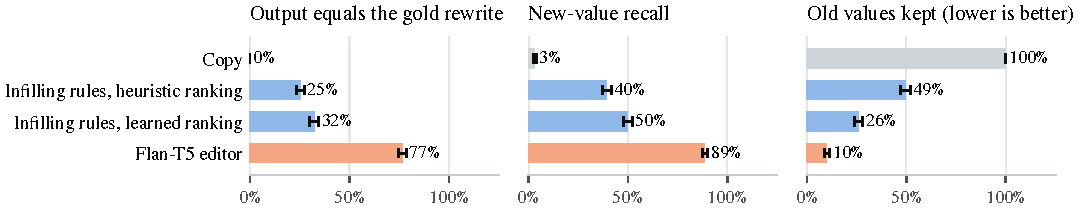
\includegraphics[width=0.78\textwidth]{figures/values.pdf}
\caption{Value-level scores on the supported test \edit{} sentences: exact match, new-value recall and old values kept.}
\label{fig:values}
\end{figure*}

\begin{table}[H]
\centering
\small
\setlength{\tabcolsep}{5pt}
\resizebox{\columnwidth}{!}{%
\begin{tabular}{@{}lcccc@{}}
\toprule
\textbf{Detector} & \textbf{Casc. R-L} & \textbf{Casc. recall} & \textbf{Upd. R-L} & \keep{} \textbf{verb.} \\
\midrule
Single round & 0.210 & & 0.436 & 92.9\% \\
Mention overlap & & 28.9\% & & \\
Staleness delta & 0.270 & 13.8\% & 0.448 & 86.7\% \\
Edited as evidence & 0.276 & 72.0\% & \textbf{0.476} & 84.0\% \\
Consequence loop & \textbf{0.296} & \textbf{79.3\%} & 0.470 & \textbf{89.8\%} \\
\midrule
Consequence loop, gold labels & 0.339 & & 0.514 & 100.0\% \\
\bottomrule
\end{tabular}%
}
\caption{The loop with each cascade detector on the 220 linked test articles. The single round has no detector, and the gold labels include the cascade sentences, so neither row has a detector recall. Mention overlap, which flags a sentence that shares a name or number with a repaired sentence, was run only in the recall test. Bold marks the best of the three detectors.}
\label{tab:cascade_results}
\end{table}

\begin{table}[tb]
\centering
\small
\setlength{\tabcolsep}{5pt}
\resizebox{\columnwidth}{!}{%
\begin{tabular}{@{}lrccccc@{}}
\toprule
\textbf{Tokens} & \textbf{Count} & \textbf{On new value} & \textbf{Uniform} & \textbf{Top token} & \textbf{Top passage} & \textbf{Null} \\
\midrule
Stale & 5,284 & \textbf{0.395} & 0.055 & \textbf{63.9\%} & \textbf{76.3\%} & 0.0002 \\
\quad new value a year & 1,220 & 0.443 & 0.055 & 81.6\% & & 0.0003 \\
\quad new value a number & 355 & 0.421 & 0.048 & 73.5\% & & 0.0003 \\
\quad new value a name & 3,709 & 0.377 & 0.056 & 57.1\% & & 0.0002 \\
Not stale & 37,879 & 0.138 & 0.040 & 22.7\% & 53.5\% & 0.0005 \\
\bottomrule
\end{tabular}%
}
\caption{Where the attention weight of the staleness classifier falls on the test split. On new value is the share of weight on the tokens of the gold new value, Uniform the share those tokens hold among the evidence tokens, Top token the share of tokens whose largest weight is on a new-value token, Top passage the share whose most weighted passage holds the new value, and Null the share of weight on the null slot. Bold marks the higher of stale and not-stale tokens.}
\label{tab:focus}
\end{table}

\begin{table}[tb]
\centering
\small
\setlength{\tabcolsep}{5pt}
\resizebox{\columnwidth}{!}{%
\begin{tabular}{@{}llcc@{}}
\toprule
\textbf{Axis} & \textbf{Run} & \textbf{ROUGE-L} & \textbf{Difference to copy} \\
\midrule
\multirow{4}{*}{Masks}
  & Oracle masks, no infilling rules & \textbf{0.912} & $\mathbf{+0.037}$ \\
  & Oracle masks, no infilling rules, no evidence & 0.854 & $-0.021$ \\
  & Linear masks, no infilling rules & 0.876 & $+0.001$ \\
  & Attention masks, no infilling rules & 0.884 & $+0.009$ \\
\midrule
\multirow{3}{*}{Ranking}
  & Infilling rules, heuristic ranking & 0.912 & $+0.038$ \\
  & Infilling rules, learned ranking & 0.929 & $+0.054$ \\
  & Flan-T5 editor & \textbf{0.973} & $\mathbf{+0.098}$ \\
\midrule
\multirow{6}{*}{Infilling rules}
  & No edit penalty & & $-0.008$ \\
  & No rejection rule & & $-0.005$ \\
  & No span cap & & $-0.000$ \\
  & No evidence veto & & $-0.002$ \\
  & No evidence-copy candidates & & $-0.004$ \\
  & All infilling rules, learned ranking & & $\mathbf{+0.012}$ \\
\bottomrule
\end{tabular}%
}
\caption{Single-round ablations. The mask and ranking rows are scored on the 1,670 supported test \edit{} sentences, with the difference to copy. The infilling-rule rows remove one rule at a time on the 300-article sample, with the difference to the setting that has all of them. Bold marks the best run of each group.}
\label{tab:ablation-single}
\end{table}

\section{Ablations}
\label{sec:ablations}

Table~\ref{tab:ablation-single} changes one part of the repair step at a time, and Table~\ref{tab:matched} holds the stress sets.

\paragraph{Infilling Rules}
Removing the edit penalty, the rejection rule or the evidence veto lowers the sentence score, and the paired bootstrap interval of each difference excludes zero. The intervals of the span cap and of the evidence-copy candidates cover zero on the sample (Table~\ref{tab:ablation-single}). On the 901 articles the infilling rules lower UpdateROUGE-L from 0.793 to 0.601 and the unsupported mentions per article from 1.02 to 0.26.

\paragraph{Ranking}
On the full test set the learned ranking gains 0.016 over the heuristic ranking, with a 95\% paired interval of 0.013 to 0.020, and it also gains under oracle masks on the 300-article sample (Table~\ref{tab:ablation-single}).

\paragraph{Stress Sets}
On 200 validation articles with the passages that state the new value removed for half of the \edit{} sentences, the infilling rules score as copy. With one added passage per \edit{} sentence that mentions the old value in another context, they score below copy. The editor keeps about half of its gain over copy on the missing-value set and most of it on the old-value set (Table~\ref{tab:matched}).

\begin{table}[tb]
\centering
\small
\setlength{\tabcolsep}{5pt}
\resizebox{\columnwidth}{!}{%
\begin{tabular}{@{}lrrrrr@{}}
\toprule
\textbf{Split} & \textbf{Articles} & \keep{} & \edit{} & \drop{} & \textbf{Linked} \\
\midrule
Train & 12,180 & 27,061 & 12,360 & 3,062 & 1,589 \\
Validation & 1,564 & 3,472 & 1,575 & 414 & 198 \\
Test & 1,602 & 3,500 & 1,684 & 428 & 220 \\
\bottomrule
\end{tabular}%
}
\caption{Articles, sentence labels and articles with a cascade link per split.}
\label{tab:splits}
\end{table}


\section{Compute}
Every run used one NVIDIA A100 with 40~GB of memory, rented by the hour, because LLaDA-8B-Base in bfloat16 holds 16~GB of weights and the cache of hidden states that the classifiers train on is over 100~GB, above the storage quota of the shared cluster available to the authors. At INR 84.24 per hour, the grant of INR 5,880 buys about 70 A100 hours. The initial experiments on FRUIT took about 37 of these hours, the experiments on Wiki Wrong about 25, and about 7 remain unspent.


\end{document}
